\chapter*{Abstract}

%TODO rewrite abstract

%This is context (says art):
I wonder: why, in the richest of countries, in the most enlightened of times (current day \gls{OECD}-world), are our welfare states so constrained and inefficient, our democracies so confused and distorted? 
	%do I mean something specific/scientific by these adjectives?
	%you should cite some previous author, literature on here (you'll pick your reviewer!, also, you really need to give credit! says Art).
	%say what you're problem is with the mainstream literature. Don't say criticize.
	%So far, this question has been answered by looking at welfare state spending and revenue. %However, ...
	%However, this work would benefit from alternative configurations of welfare states and democracies, and for failing to explain their absence. %put something equally concrete as spending and revenue, examine the tax law itself.
	%explain welfare state retrenchment
	%include the whole progression thing earlier
	%stress that this is an experiment, which isn't so common otherwise (this would make it sexy) (include control groups)
	%maybe include the questionnaire, do pre/post, 4-5 days, 
	%absolutely stress the sense of validity
I ask: if a hypothetical, superior political process (deliberative democracy) ruled our polity, would we think better and fairer about the institutions of the mixed economy and would we opt for a hypothetical, superior tax regime (\gls{PCT}, \gls{LVT} and \gls{NIT})? 

And so I test: if given the possibility to deliberate well-informed, fairly and thoroughly (a deliberative poll), will randomly selected, ordinary voters understand the mixed economy differently (better) and prefer a different tax (\gls{PCT}, \gls{LVT} and \gls{NIT})? %control group
		
	%We hope that people will understand and prefer [use same concepts as above, link] a more progressive and efficient tax
			
If, in fact, they do, welfare state research will have a lot more to explain, and deliberative democracy will have shown its stripes.

\begin{figure}[htbp]
	\centering
	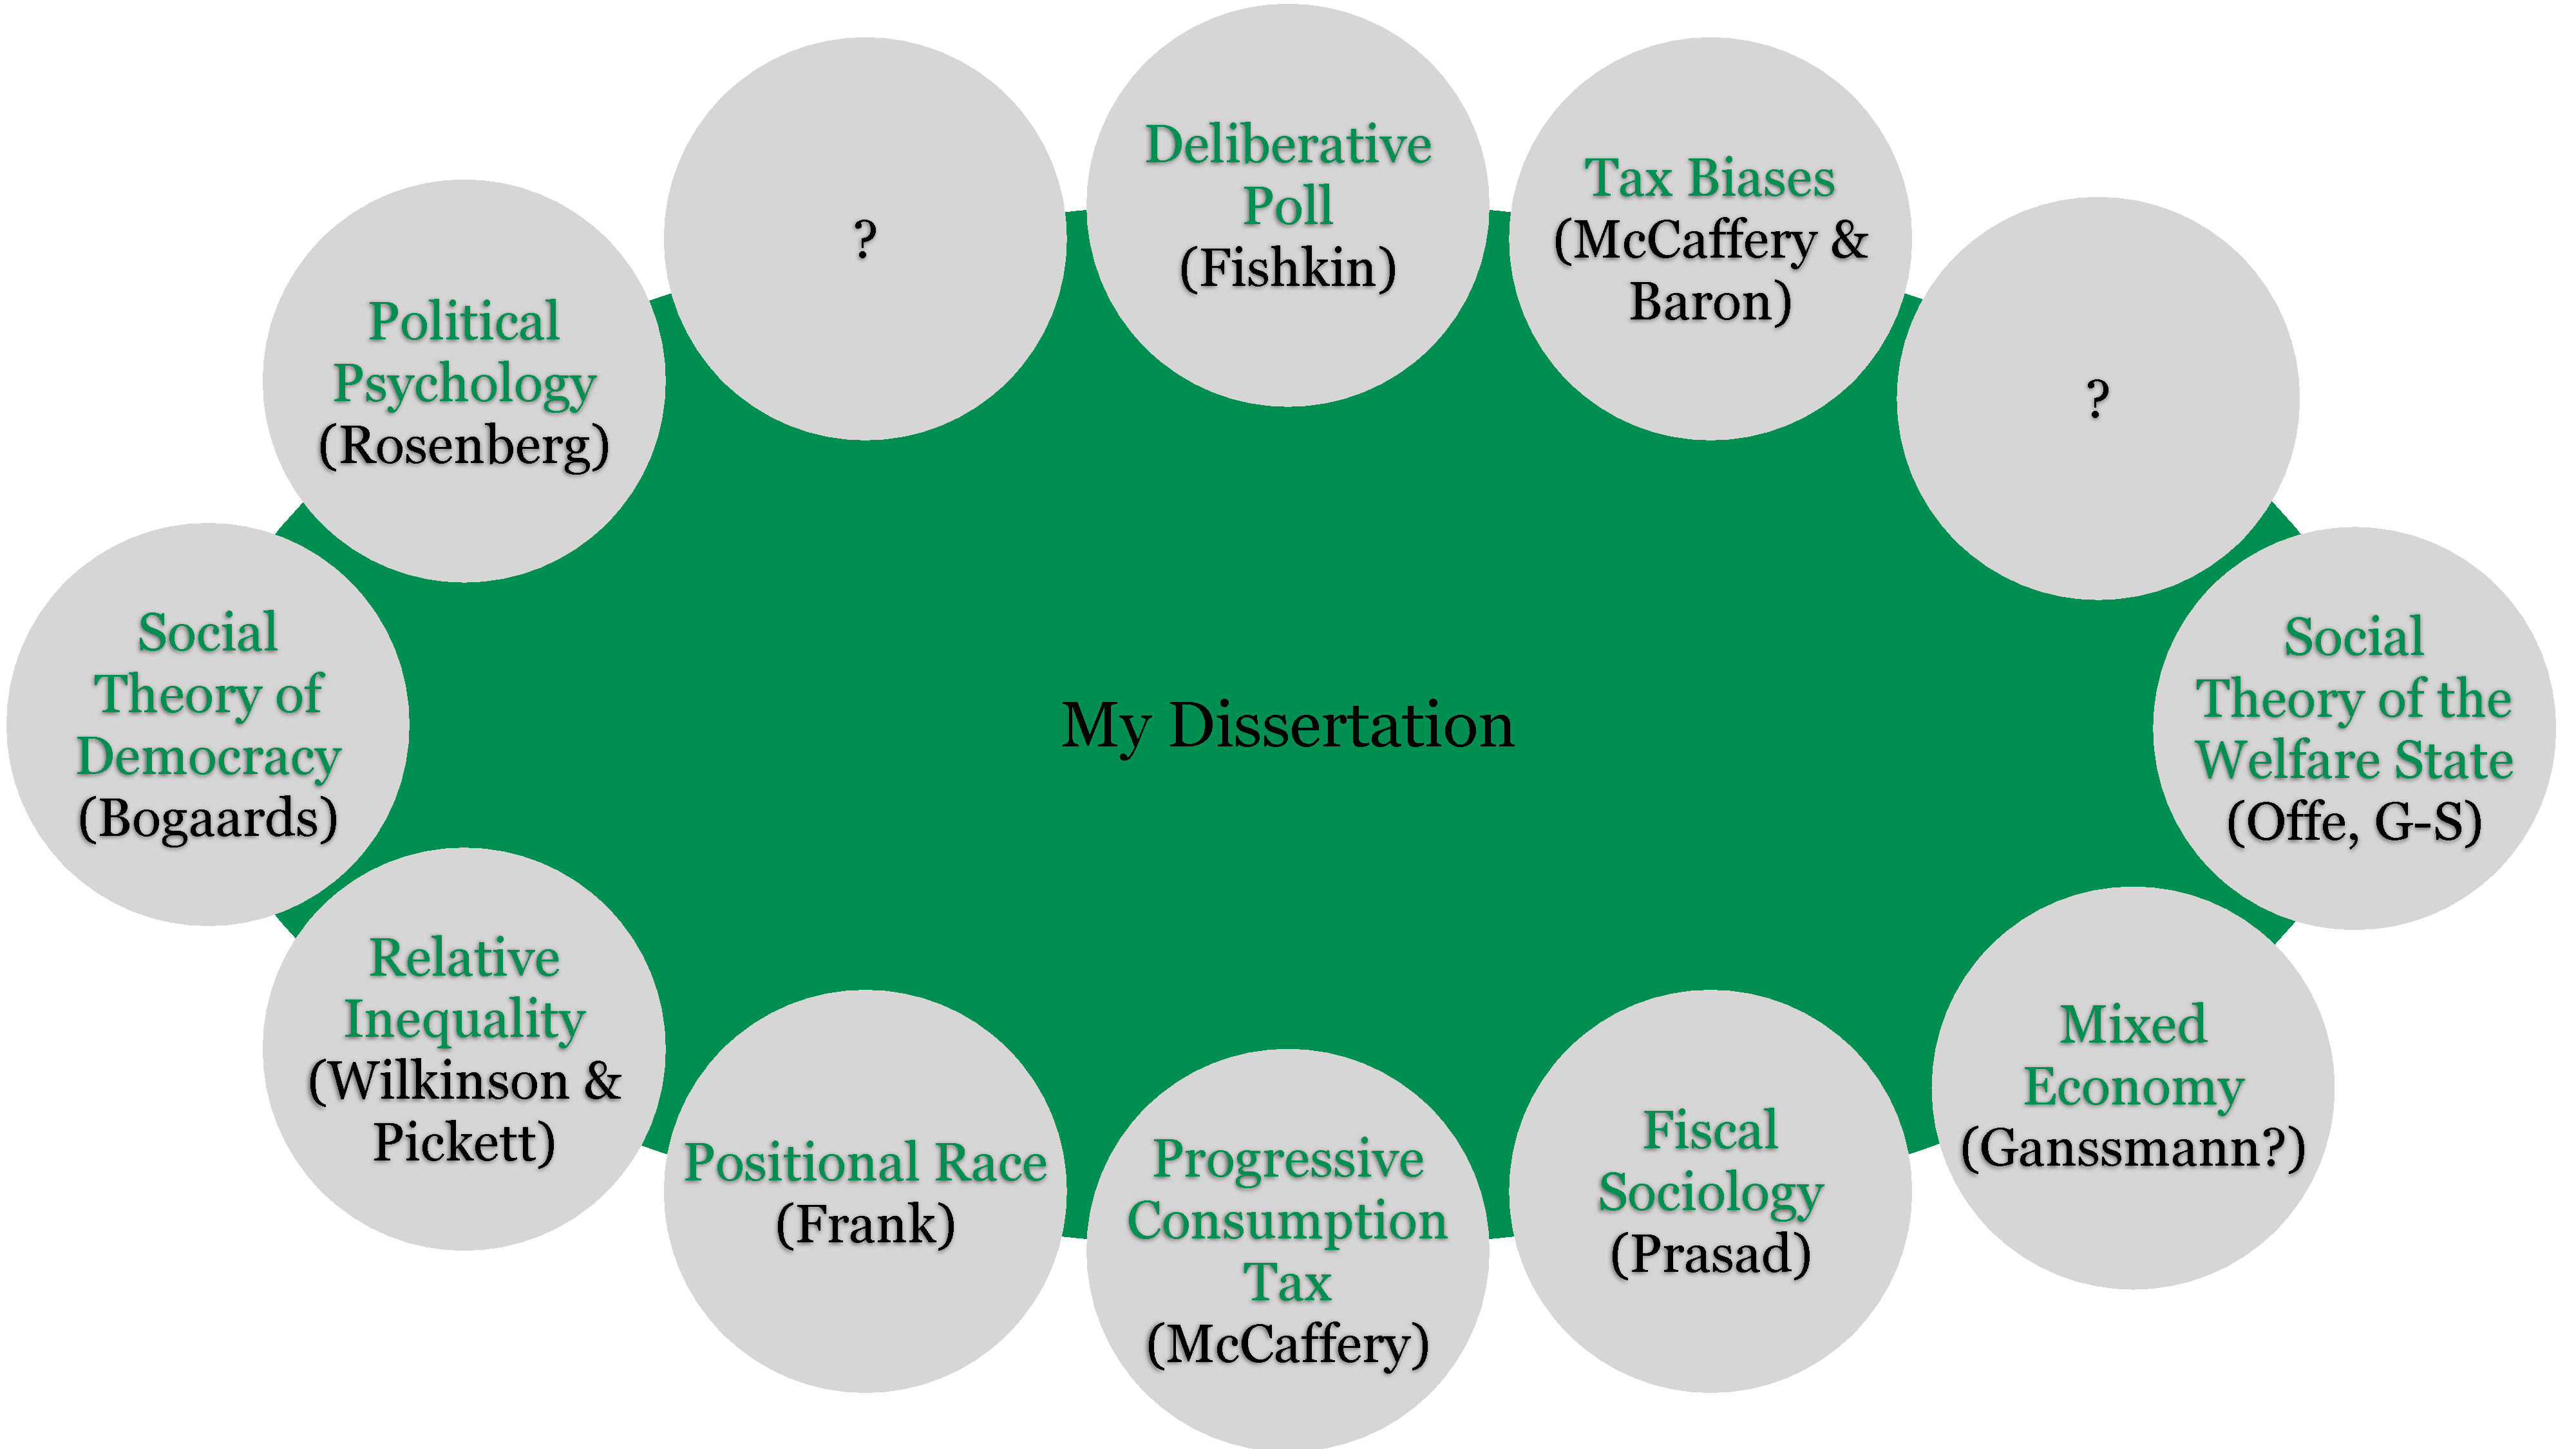
\includegraphics[width=1\linewidth]{diss-expertise}  
	\caption{Academic Fields and Advisors for this Dissertation}
	\label{fig:diss-expertise}
\end{figure}

\begin{landscape}
\begin{figure}[htbp]
	\centering
	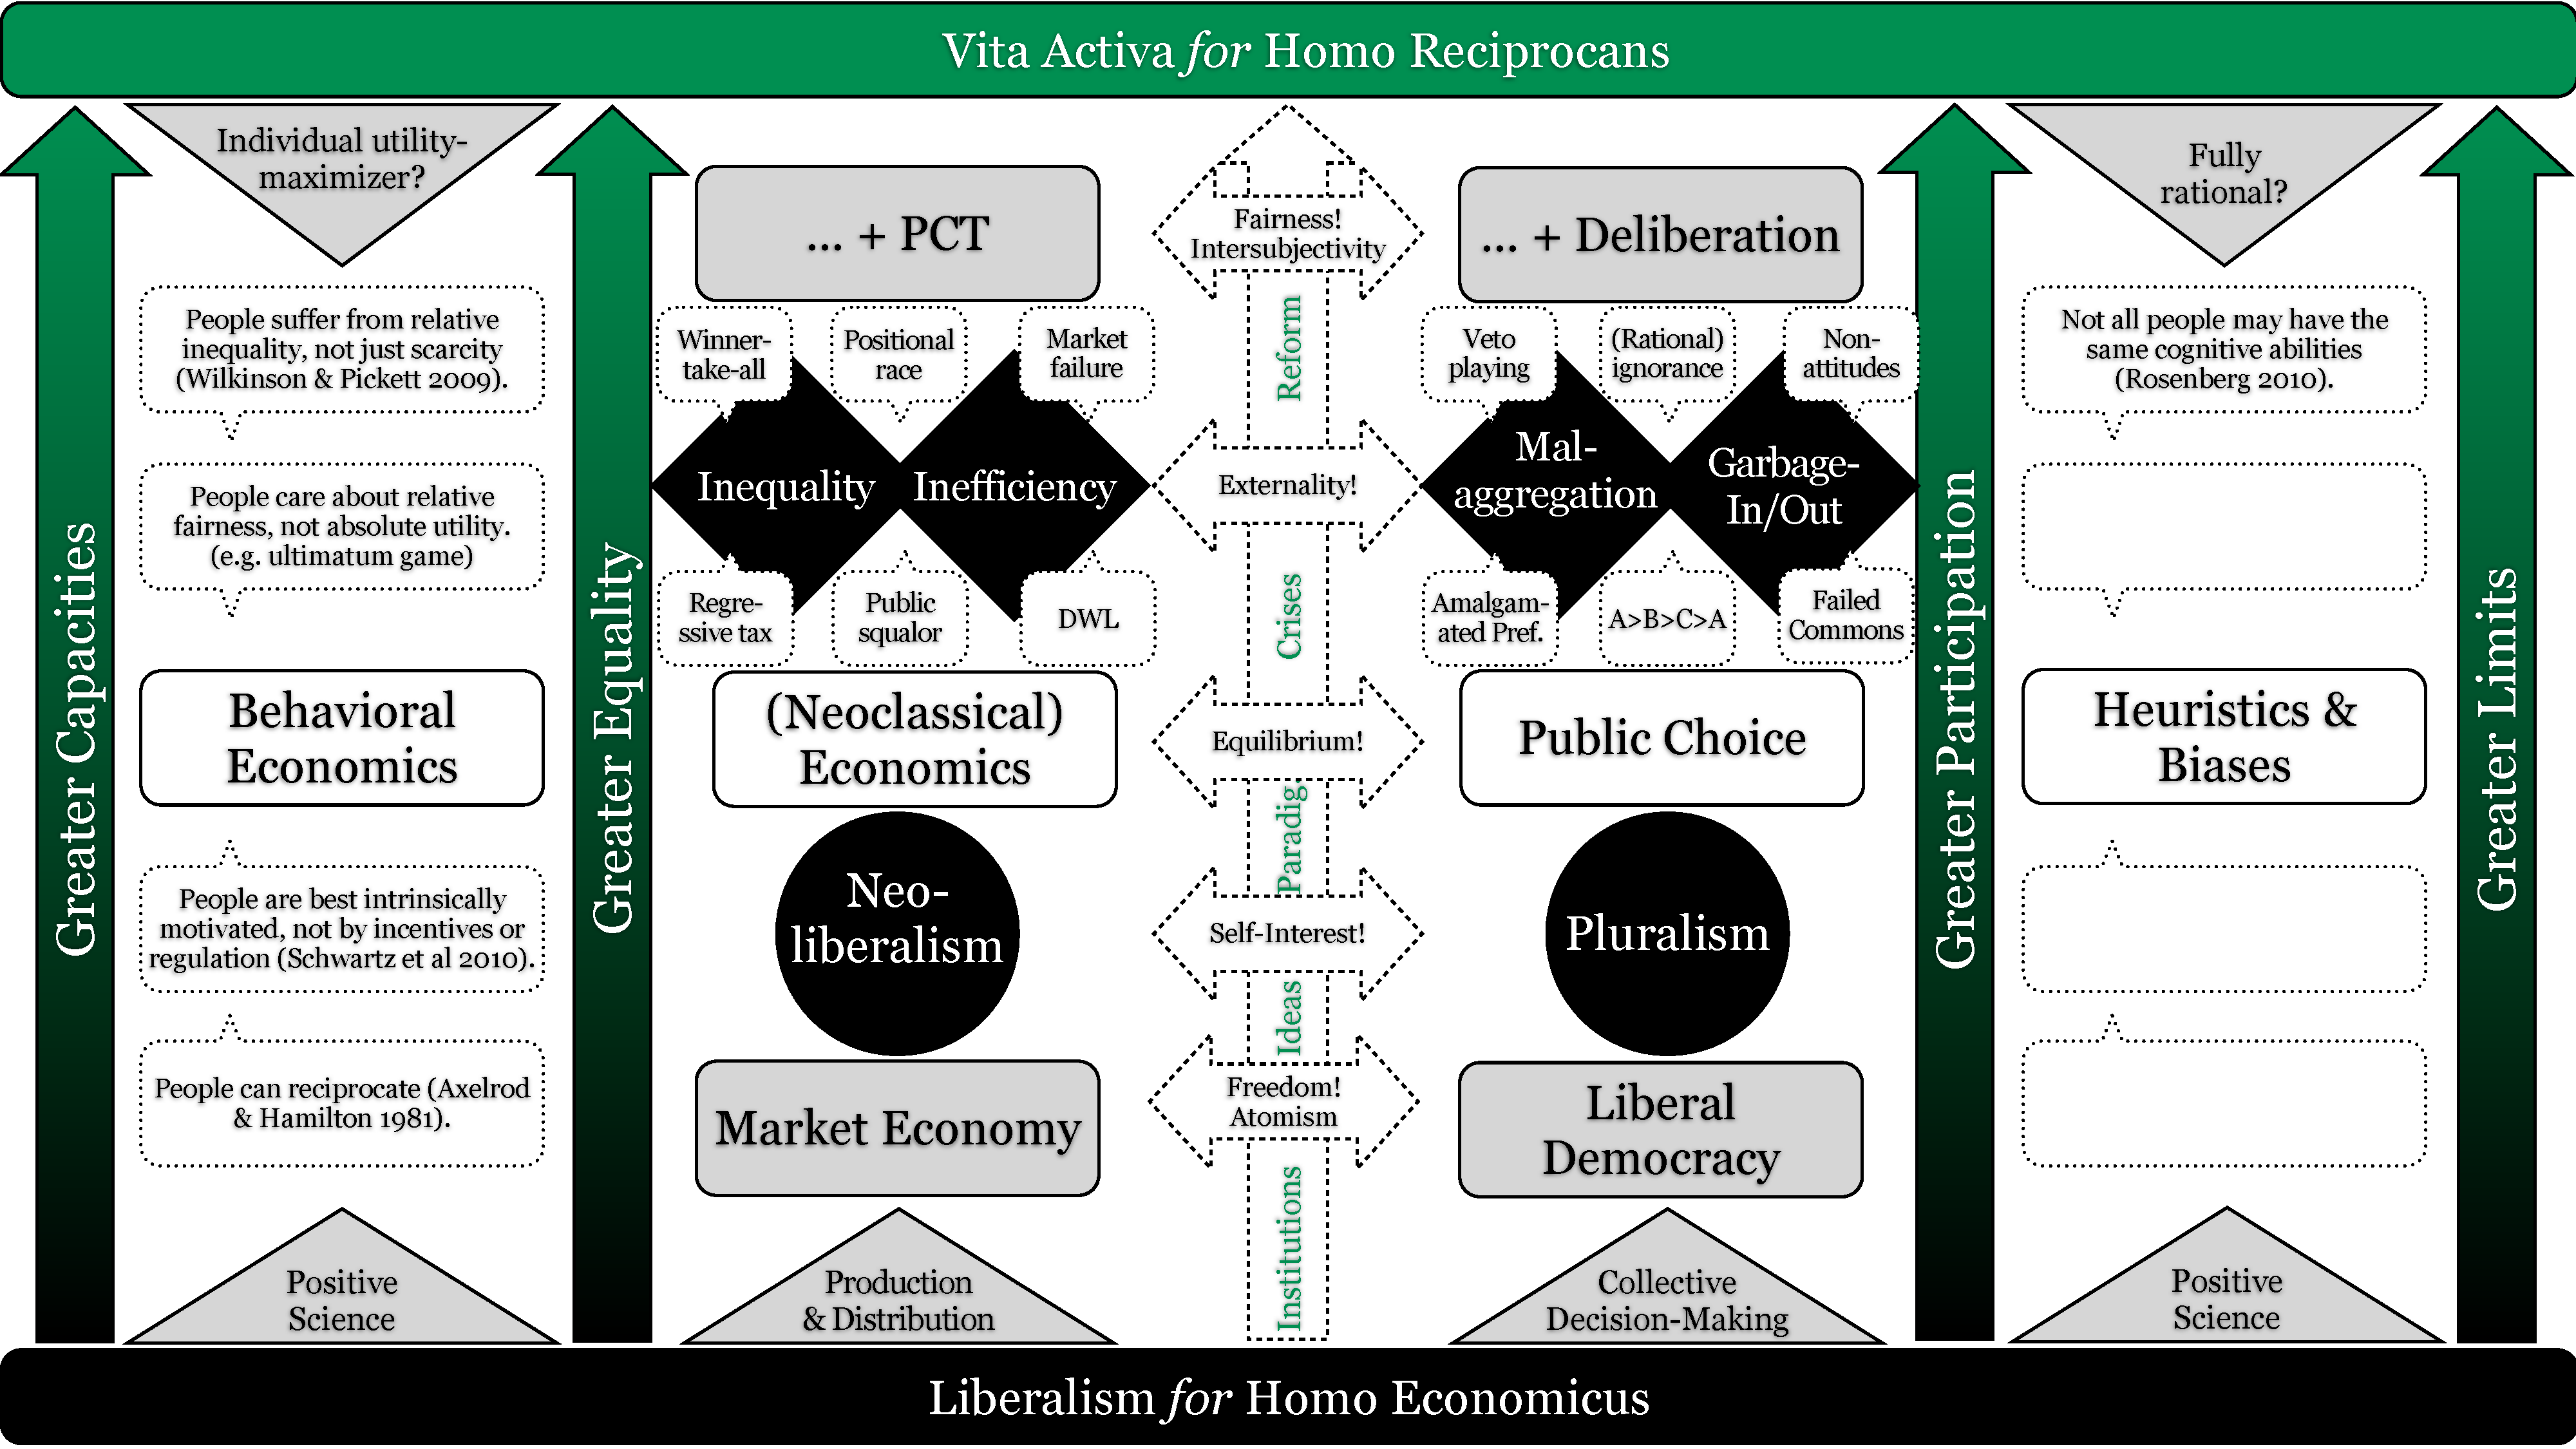
\includegraphics[width=1\linewidth]{diss-mindmap}  
	\caption{Mindmap of this Dissertation}
	\label{fig:diss-mindmap}
\end{figure} 
\end{landscape}